Wir stellten die Spannungen $U_{FR}$, $U_{KA}$ und $U_{FA}$ auf die folgenden Werte ein:

\begin{tabular}{l l l}
$U_{FR}$ & = $113\pm 2$ V & (Beschleunigungsspannung)\\
$U_{KA}$ & = 0V & (Glühkathode)\\
$U_{FA}$ & = $106\pm 0,5$V & (Massenfilters)\\
\end{tabular}

Diese Werte wurden während der folgenden Messung bis zur Bearbeitung der letzten Aufgabe nicht mehr verändert. 
Es gelang uns, den Druck während den Messungen konstant zu halten.

\subsection{Restgas-Messung}
Bei dieser Messung machten wir uns mit dem LabView-Programm vertraut und stellten die Verstärkung auf $10^{-10}$. Der Druck betrug dabei $8,9 \cdot 10^{-6}$ mbar. Zudem schlossen wir Ventil V3, öffneten das Ventil V4 und nahmen die Messung von dem Restgas. In Abb. 5 und in Tab. 1 werden die Ergebnisse dieser Messung dargestellt. Aus [4] und anhand der Periodentabelle wissen wir, dass der Peak bei m/q=18 für den Wasseranteil in dem Gas steht.

\myImage[7cm]{img/RGbalk}{Überarbeitete Daten aus der Restgasmessung}

\begin{center}
\begin{tabular}{c|c|c}
m/q [u/e] & p [$10^{-7} mbar$] & Ionen\\	
\hline	
12,5 &	0,16 & - \\
14,5 &	0,26 & $N_2$\\
16,4 &	2,20 & $O_2$\\
17,3 &	15,09 & $H_2O$\\
18,3 &	59,33 & $H_2O$ Peak\\
20,3 &	0,49 & Argon\\
26,3 &	0,73 & Ethanol\\
27,3 &	1,19 & Ethanol\\
28,2 &	8,33 & $N_2$ Peak\\
31,3 &	0,59 & Ethanol Peak\\
32,2 &	0,15 & $O_2$ Peak\\
42,2 &	0,48 & $CO_2$ Peak\\
\end{tabular}
\end{center}
\captionof{table}{Ergebnisse der Messung von dem Restgas bei einem Druck von $8,9\cdot 10^{-6}mbar$ mit errechneten Partialdrücke p und Zuordnung zu Ionen}

\subsection{Testgas 1 - Dosierung und Messung}
Über die Ventile wurde das Testgas (in diesem Fall Argon) in die Vorkammer gelassen. Anschließend starteten wir das Messprogramm und nahmen die Werte auf. Nun leerten wir den Rezipienten wieder und warteten dann 10 Minuten. Diesen Vorgang wiederholten wir für alle Messungen\\
Die Zuordnung zu den Ionen erfolgte durch [4] und mithilfe des Periodensystems der Elemente. Die Ergebnisse sind in Abb. 6 und in Tab. 2 dargestellt:\\

\myImage[9cm]{img/AGbalk}{Massenspektrum von Argon}

\begin{center}
\begin{tabular}{c|c|c}
m/q [u/e] & p [$10^{-7} mbar$] & Ionen\\	
\hline	
2,6 & 0,03	&\\	
14,0 & 0,18	&\\	
14,8 & 0,21	&\\	
16,4 & 0,50	&\\	
17,3 & 4,39	&\\	
18,3 & 17,71 & $H_2O$ Peak\\
20,3 & 0,42	& Argon\\
25,7 & 0,20	&\\
26,8 & 0,17	&\\
28,3 & 2,11	& $N_2$ Peak\\
40,2 & 11,51 & Argon Peak\\
42,2 & 0,16	&\\
43,3 & 0,06	&\\
44,2 & 0,19	&\\
58,3 & 0,18	&\\
\end{tabular}
\end{center}
\captionof{table}{Ergebnisse der Messung von Argon bei einem Druck von $4,0\cdot 10^{-6}mbar$ mit errechneten Partialdrücke p und Zuordnung zu Ionen}

\subsection{Testgas 2, 3 und Luft - Dosierung und Messung}
Bei der Messung dieser Gase sind wir wie oben beschrieben vorgegangen. Die Ergebnisse dieser Messungen werden in den folgenden Abbildungen 7, 8 und 9, sowie in den Tabellen 3, 4 und 5 dargestellt.

\myImage[9cm]{img/ACbalk}{Massenspektrum von Aceton}

\begin{center}
\begin{tabular}{c|c|c}
m/q [u/e] & p [$10^{-7} mbar$] & Ionen\\	
\hline	
2,9 &	0,77 &\\
13,0 &	0,28 &\\
14,4 &	0,97 & Aceton\\
16,4 &	2,25 &\\
17,3 &	5,84 & $H_2O$\\
18,3 &	23,09 & $H_2O$ Peak\\
21,7 &	0,35 & Argon\\
26,3 &	0,80 & Aceton\\
27,3 &	0,90 & Aceton\\
28,3 &	11,22 & Aceton, $N_2$ Peak\\
29,9 &	0,077 & Aceton\\
30,8 &	0,28 &\\
31,7 &	0,22 &\\
39,3 &	0,23 & Aceton\\
39,8 &	0,18 & Argon Peak\\
41,3 &	0,22 & Aceton\\
42,3 &	0,41 & Aceton\\
43,3 &	6,57 & Aceton Peak\\
44,1 &	0,95 &\\
45,0 &	0,24 &\\
45,9 &	0,35 &\\
58,3 &	0,80 &\\
\end{tabular}
\end{center}
\captionof{table}{Ergebnisse der Messung von Aceton bei einem Druck von $5,7\cdot 10^{-6}mbar$ mit errechneten Partialdrücke p und Zuordnung zu Ionen}

\myImage[10cm]{img/ETHbalk}{Massenspektrum von Ethanol}

\begin{center}
\begin{tabular}{c|c|c}
m/q [u/e] & p [$10^{-7} mbar$] & Ionen\\	
\hline	
2,6 &	0,17 &\\
14,4 &	0,64 & Ethanol\\
15,4 &	3,04 & Ethanol\\
16,4 &	1,90 &\\
17,4 &	5,56 & $H_2O$\\
18,4 &	22,11 & $H_2O$ Peak\\
20,0 &	0,24 &\\
24,7 &	0,38 & Ethanol\\
26,3 &	0,57 & Ethanol\\
27,3 &	0,66 & Ethanol\\
28,3 &	9,09 & Ethanol\\
30,1 &	0,16 & Ethanol\\
30,7 &	0,33 & Ethanol\\
31,7 &	0,327 & Ethanol Peak\\
39,8 &	0,25 &\\
41,3 &	0,13 &\\
42,3 &	0,31 & Ethanol\\
43,3 &	5,90 & Ethanol\\
44,1 &	0,84 & Ethanol\\
45,8 &	0,39 & Ethanol\\
\end{tabular}
\end{center}
\captionof{table}{Ergebnisse der Messung von Ethanol bei einem Druck von $5,0\cdot 10^{-5}mbar$ mit errechneten Partialdrücke p und Zuordnung zu Ionen}

\myImage[10cm]{img/Luftbalk}{Massenspektrum von Luft}

\begin{center}
\begin{tabular}{c|c|c}
m/q [u/e] & p [$10^{-7} mbar$] & Ionen\\	
\hline	
2,6 &	0,20 &\\
14,4 &	1,41 & $N_2$\\
15,0 &	0,08 &\\
16,4 &	1,62 & $O_2$\\
17,3 &	5,31 & $H_2O$\\
18,3 &	17,71 & $H_2O$ Peak\\
19,8 &	0,20 &\\
25,5 &	0,29 &\\
27,4 &	0,48 &\\
28,2 &	26,52 & $N_2$ Peak\\
30,2 &	0,39 & $N_2$\\
30,8 &	0,15 &\\
40,2 &	0,13 & $O_2$ Peak\\
40,8 &	0,23 &\\
42,0 &	0,23 &\\
42,6 &	0,28 &\\
44,2 &	0,48 &\\
\end{tabular}
\end{center}
\captionof{table}{Ergebnisse der Messung von Luft bei einem Druck von $5,6\cdot 10^{-6}mbar$ mit errechneten Partialdrücke p und Zuordnung zu Ionen}

\newpage
\subsection{Auflösungsvermögen des Spektrometers}
Aus Gl. 8 ist bekannt:

\begin{equation}
\notag
b = \frac{2qV}{mr_{0}^{2}\omega^{2}}
\end{equation}

Daraus folgt für m:

\begin{equation}
m = \frac{2qV}{br_{0}^{2}\omega^{2}}
\end{equation}

Wenn wir nun zwei Punkte auf der Arbeitsgeraden haben, ergibt sich bei einer konstanten Spannung die Breite des Massenpeaks:

\begin{equation}
\Delta m = \frac{2qV}{r_{0}^{2}\omega^{2}}\cdot \left( \frac{1}{b_1}-\frac{1}{b_2}\right) \qquad \text{mit} \qquad b_1 < b_2
\end{equation}

Nehmen wir nun an, dass sich die gemessenen Massen in der Mitte der Peaks befinden, dann gilt für b:

\begin{equation}
b = \frac{b_1 + b_2}{2}
\end{equation}

Daraus folgt:

\begin{equation}
\frac{b_1 + b_2}{2}=\frac{2qV}{mr_0^2 \omega^2} \leftrightarrow m = \frac{2qV}{r_0^2 \omega^2}\cdot \frac{2}{b_1 + b_2}
\end{equation}

Und somit für m/$\Delta$ m:

\begin{equation}
\frac{m}{\Delta m} = \frac{2}{(b_1+b_2)\cdot \left(\frac{1}{b_1}-\frac{1}{b_2}\right)} = \frac{2}{\frac{b_2}{b_1}-\frac{b_1}{b_2}}
\end{equation}

Man kann also von einer konstanten Massenauflösung ausgehen. Geht man davon aus, dass $\Delta$m mit der Beschleunigungsspannung zusammenhängt, ergibt sich für Ionen im Filter eine Geschwindigkeit von:

\begin{equation}
v=\sqrt{\frac{2qU_B}{m}}
\end{equation}

Je höher die Beschleunigungsspannung ist, desto kürzer ist die Aufenthaltsdauer im Massenfilter und desto geringer ist die Genauigkeit. Daraus folgt für die Anzahl $n$ der Durchlaufenen Schwingungen:

\begin{equation}
n = \frac{f\cdot l}{v}= f\cdot l \cdot \sqrt{\frac{m}{2qU_B}}
\end{equation}

mit der Frequenz $f$ und der Länge $l$ des Massenfilter.\\
Es wurden zwei Messungen mit Luft als Testgas durchgeführt, um diese Relationen zu untersuchen. Dabei variierte bei der ersten Messung der Wert von $a$ und bei der Zweiten der Wert von $U_{FA}$.

\begin{figure}[h]
\centering
\begin{subfigure}{0.49\textwidth}
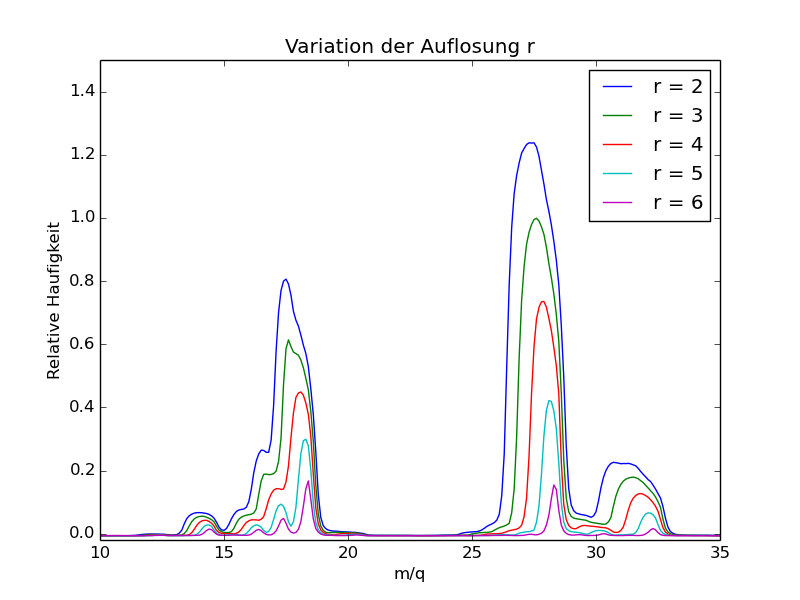
\includegraphics[width=\textwidth]{img/VAR}
\caption{Messung des Massenspektrums für Luft unter Variation der Auflösung a}
\end{subfigure}
\begin{subfigure}{0.49\textwidth}
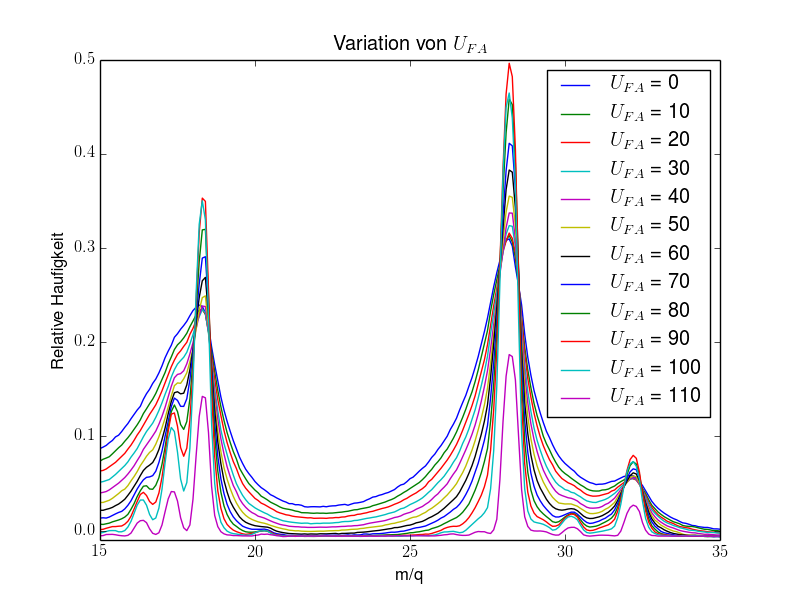
\includegraphics[width=\textwidth]{img/Ufa}
\caption{Messung des Massenspektrums für Luft unter Variation der Spannung $U_{FA}$}
\end{subfigure} 
\end{figure}

\begin{center}
\begin{minipage}{0.25\textwidth}		
\begin{tabular}{l|l|l}
a & m/q & $\Delta m$\\	
\hline		
2 & 27,45 & 2,20\\
3 & 27,62 & 1,99\\
4 & 27,90 & 1,17\\
5 & 28,19 & 0,69\\
6 & 28,35 & 0,33\\
\end{tabular}
\end{minipage}
\begin{minipage}{0.25\textwidth}
\begin{tabular}{l|l|l}
a & m/q & $\Delta m$\\
\hline
2 &	31,37 &	2,49\\
3 & 31,49 &	1,90\\
4 & 31,77 &	1,29\\
5 & 32,18 &	0,72\\
6 & 32,34 &	0,36\\
\end{tabular}
\end{minipage}
\captionof{table}{Werte aus Abb. 10 mit bestimmtem $\Delta m$ für den Peak bei m/q = 28 (Stickstoff) und bei m/q = 32 (Sauerstoff) mit der FWHM-Methode}
\end{center}

\begin{figure}[h]
\centering
\begin{subfigure}{0.49\textwidth}
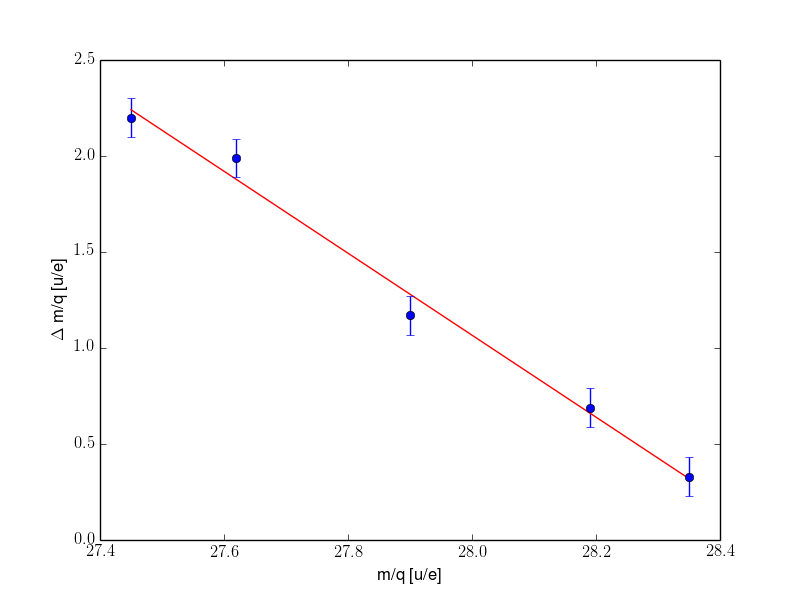
\includegraphics[width=\textwidth]{img/mq1}
\end{subfigure}
\begin{subfigure}{0.49\textwidth}
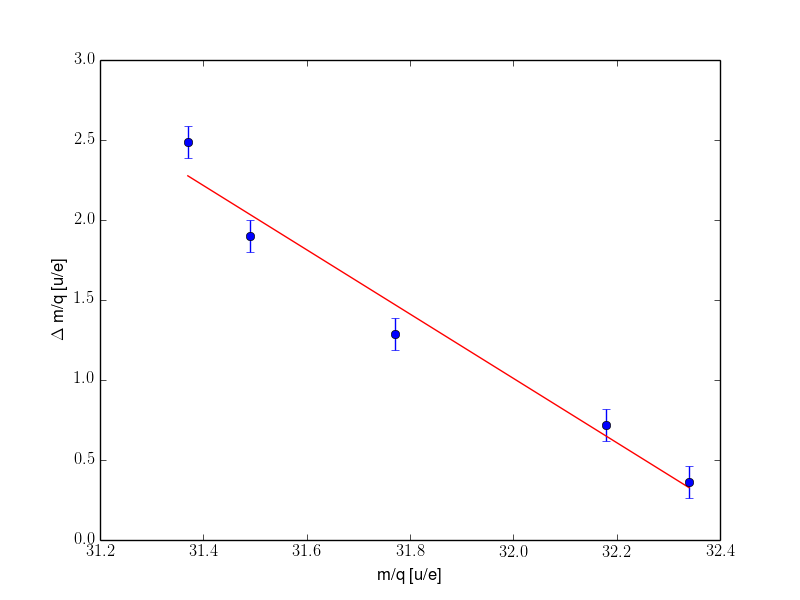
\includegraphics[width=\textwidth]{img/mq2}
\end{subfigure} 
\caption{Lineare Regressionen der Daten aus Tabelle 6. Die Fehler wurden durch die Gauß’schen Fehlerfortpflanzung ermittelt. Dafür schätzten wir den Ablesefehler $\Delta(m/q)$ auf 0.1[u/e]. Die Steigungen betragen $2,07\pm 0,14$.}
\end{figure}

Für die Erstellung von Abb. 12 wurde angenommen, dass die Massen sich in der Mitte der Peaks befinden. Dadurch konnten wir die FWHM-Methode anwenden. Es ist erkennbar, dass die Variation der Auflösung nichts am Verhältnis zwischen $\Delta$m und m ändert. Lediglich der Wert von m/q verschiebt sich und die Anzahl der Ionen, welche am Detektor eintreffen, sinkt. Anders ist es, wenn man $U_{FA}$ verändert. Dabei bleibt der m/q-Wert stabil und die Peaks der einzelnen Messungen nähern sich einander an (siehe Abb. 14). Bei dieser Auswertung gingen wir von den selben Voraussetzungen wie oben  aus. Für die Beschleunigungsspannung gilt $U_{B} = U_{FR}-U_{FA}$ und daraus folgt für die Anzahl der Schwingungen der Ionen aus Gl. 16, dass die Aufenthaltsdauer im Massenfilter für kleine $U_{FA}$ klein ist. Die Frequenz wurde für die Rechnungen auf 2,5MHz festgelegt und die Länge des Spektrometers betrug 0,1m. Die errechneten Werte für die $\Delta$m/q wurden in Abb. 14 über die Anzahl der Schwingungen $n$ aufgetragen. Im Rahmen der Ablesegenauigkeit von 0,1[U/e], verhalten sich die Werte wie in Tab. 6, sind also identisch.

\myImage[10cm]{img/delta_m_n}{Darstellung der Halbwertsbreiten über der Anzahl der Schwingungen. Der Fehler wurde auf 0.1u/e geschätzt.}

\section{Zusammenfassung und Diskussion}
In diesem Versuch wurde mit einem Quadrupolmassenspektrometer die Spektren von Argon, Aceton, Ethanol und Luft, aufgenommen und untersucht. Die Durchführung verlief reibungslos und es traten keine Probleme auf.\\
In den einzelnen Spektren wurden jeweils die erwarteten Ionen entdeckt. Die theoretische Herleitung des Auflösungsvermögens lieferte den erwarteten konstanten Zusammenhang zwischen m und $\Delta$m.\\
In der Auswertung wandten wir die FWHM-Methode an um die Spektren der Luft unter Variation der Auflösungen und der Spannung $U_{FA}$. Da wir aber nur annahmen, die Massen in der Mitte der Peaks zu finden, ist das eine ungenaue Methode. Dennoch, oder vielleicht genau deswegen, gelangten wir mit dieser Methode zu dem Ziel, was erwartet wurde.\\
Bei der Untersuchung von Luft als Testgas, entdeckten wir ebenfalls die erwarteten Gase.\\
Zusammenfassend lässt sich also sagen, dass der Versuch erfolgreich durchgeführt wurde.